\documentclass{article}
\usepackage{graphicx} % Required for inserting images
\usepackage{amsmath}
\usepackage{indentfirst}
\usepackage[margin=0.8in]{geometry}
\usepackage[backend=biber,style=authoryear, citestyle=authoryear]{biblatex}
\addbibresource{references.bib} % your .bib file

\title{Developing a Schedule to Guide Resynchronization of Circadian Rhythms Using the Goodwin Oscillator Model}
\author{Ines de Uriarte Alvarez de Espejo, Ghazala Singh, Lia Campbell}
\date{October 3rd 2025}

\begin{document}
\maketitle

\section{Motivation and Problem}
\indent With the rise of globalization and the increasing frequency of long-term flights, jet lag has become an increasingly relevant issue for many individuals. Anyone who has rapidly crossed several time zones has experienced symptoms including fatigue, sleep misalignment and lack of focus\footcite{source1} among others. In fact, athletes always have to arrive at the site of competitions several days before the event due to jet lag\footcite{source2}.

Ultimately, jet lag is caused by a misalignment of our internal biological clock known as circadian rhythms\footcite{source1}. When there is a sudden environmental change, such as moving time zones, the body takes some time to adapt, causing jet lag. This project aims to minimize the effects caused by this misalignment by optimizing light exposure which can help realign internal biological clocks, ultimately producing a schedule for individuals.

\section{Mathematical Background}
\indent Circadian rhythms are generated by internal biological clocks that complete a full oscillation every 24 hours. These clocks are regulated by feedback loops originating from clock genes and proteins. It is known that among the external cues (zeitgebers) that affect these clocks, light is the strongest, producing phase advances in the morning and delays in the evening\footcite{source3}. Ultimately this makes light the best resynchronization for misalignments\footcite{source4}.

In order to represent circadian dynamics mathematically, we want to adopt the most widely used model: the Goodwin Oscillator Model. This three-variable non-linear ODE model is used to capture feedback between mRNA, proteins, and an inhibitory factor\footcite{source5}.

\begin{align}
\frac{dX}{dt} &= \frac{\tau'}{\tau} \left( \frac{1}{1+\left(\tfrac{Z}{K}\right)^{h}} - d_{1}X \right) + L I(t), \\[6pt]
\frac{dY}{dt} &= \frac{\tau'}{\tau} \left( X - \frac{d_{2}Y}{1+cY} \right), \\[6pt]
\frac{dZ}{dt} &= \frac{\tau'}{\tau} \left( Y - d_{3}Z \right).
\end{align}

In this model, X is mRNA, Y is a protein, and Z an inhibitor. LI(t) is light, with L calibrated so a 1h bright-light pulse produces 1 hour of advances in the morning and delays in the evening, consistent with human response curves\footcite{source6}, and I(t) being optimized to minimize the error while respecting limits on light dose and sleep protection. The rest of the parameters are set to match human free run data\footcite{source7}.

\section{Project Goal Statement}
\indent The goal of this project is to develop a computational tool that generates optimized light exposure schedules for individuals experiencing abrupt time-zone transitions. By modelling circadian rhythm dynamics using the Goodwin Oscillator Model, this tool will simulate how light exposure influences circadian phase adjustment. The optimization will minimize circadian misalignment, reduce the total required light exposure, and respect sleep windows to limit disruption. Ultimately the project aims to produce practical schedules tailored to user-specific inputs, such as flight details, to accelerate resynchronization and improve well being.

\section{Objectives}
\indent 1. Implement user interface that allows for user input about the misalignment between the user’s current and desired circadian rhythm
2. Develop an improved Goodwin Oscillator Model tailored to circadian rhythms using numerical ODE solvers 
3. Optimize for minimized circadian phase error and minimal total light dose
4. Stimulate candidate schedules under varying parameter sets and demographic considerations 
5. Visualize and analyse results by producing plots
6. Deliver outputs including quantitative comparisons of schedules and user friendly recommendations generated with a large language model (LLM)

\section{Expected Outcomes}
\indent To account for uncertainty of changes to the user’s schedule, five sets of parameters will be generated, corresponding to the circadian periods spanning a range of 2 hours around the inputted jet lag. For each parameter set, the optimal daily light exposure in hours for one week will be calculated using the Goodwin Oscillator Model. The optimization will account for minimizing circadian phase error, limiting total light exposure, and avoiding light during sleep windows. 
Using MATLAB and/or Python, a Goodwin Oscillator Model tailored to synchronization of circadian rhythms will be implemented to compute the recommended hours of daily light exposure for each parameter set. The computation will optimize for minimizing circadian phase error, limiting total light exposure, and avoiding light during sleep windows. Four candidate schedules will be drafted using a Large Language Model, with each schedule tailored to a demographic: children, the elderly, teenagers, and adults. For each schedule, the resynchronizing process will be simulated using the Goodwin Oscillator Model. The final outputs will include 1) phase plots, showing circadian trajectories relative to target alignment; 2) bifurcation diagrams exploring how changes in parameters affect stability of resynchronization; and 3) error plots showing decay of phase misalignment across time. These plots allow for comparison of the statistics of each schedule. The user will choose their preferred schedule, and have it as a guide to resynchronize their circadian rhythm.

\section{Timeline}
\indent The timeline of the project as of now is as follows:


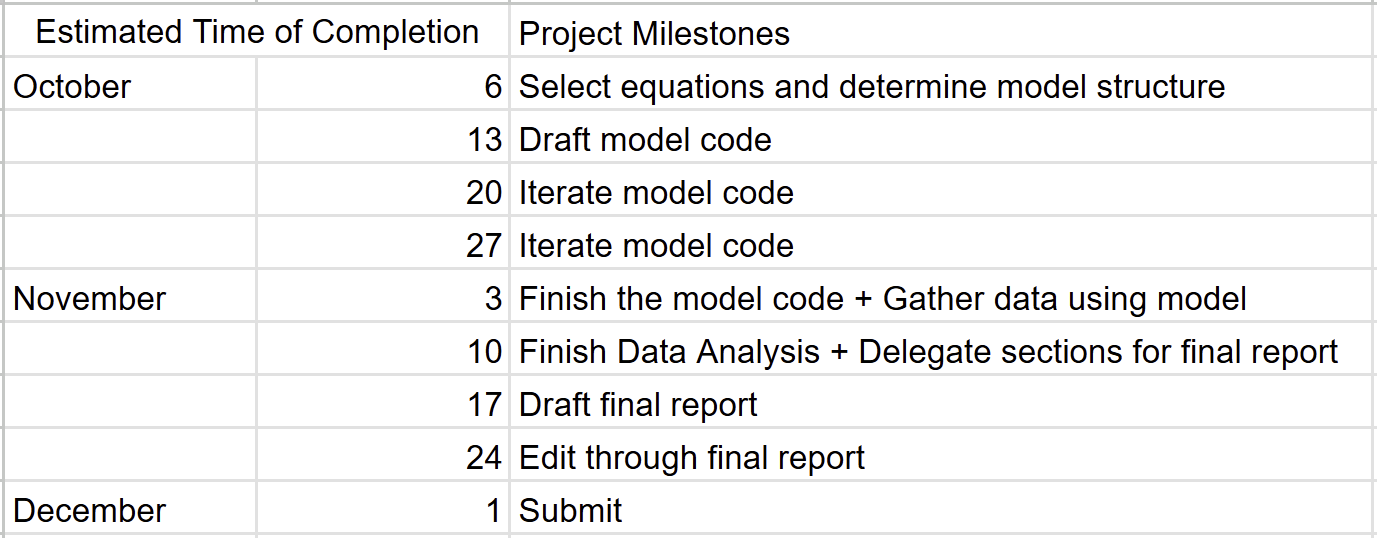
\includegraphics[scale=0.4]{timeline.png}

\section{Works Cited}
\printbibliography

\end{document}